%%%%%%%%%%%%%%%%%%%%%%%%%%%%%%%%%%%%%%%%%%%%%%%%
%%%%%%%%%%%%%Przykładowy dokument%%%%%%%%%%%%%%%
%%%%%%%%%%wraz z klasą pracadyp.cls%%%%%%%%%%%%%
%%%%%%%%%%%%%%%%%%%%%%%%%%%%%%%%%%%%%%%%%%%%%%%%

% w nawiasie kwadratowym wpisujemy rodzaj pracy: 
% magisterska, licencjacka, inzynierska
\documentclass[magisterska]{pracadypl}

%% ważne definicje %%
\usepackage{amsmath}
\usepackage{caption}
\usepackage{tabularx}
\usepackage{longtable}
\usepackage{tgtermes}
\usepackage[T1]{fontenc}
\usepackage{polski}
\usepackage[utf8]{inputenc}
\input glyphtounicode
\pdfgentounicode=1
\usepackage{amssymb}
\usepackage{amsmath}
\usepackage{graphicx}
\usepackage{titlesec}
\usepackage{color}
\usepackage{xcolor}
\usepackage{float}
\bibliographystyle{plain}

\def\mgr{magisterska}
\def\lic{licencjacka}
\def\inz{inżynierska}

\def\sk{Słowa kluczowe}
\def\kw{Keywords}
\def\et{Title in English}
%% koniec ważnych definicji %%

\usepackage{tikz}
\usetikzlibrary{shapes.geometric, arrows}
\usepackage{listings}
\usepackage{xcolor}

\lstset{ % Ustawienia dla środowiska listings
    backgroundcolor=\color{white},   % Kolor tła
    basicstyle=\footnotesize\ttfamily, % Styl podstawowy
    breaklines=true,                  % Zawijanie długich linii
    frame=single,                     % Ramka wokół kodu
    keywordstyle=\color{blue},        % Kolor słów kluczowych
    commentstyle=\color{darkgray},       % pogrubienie komentarzy
    stringstyle=\color{gray},          % Kolor stringów
    language=Python                   % Język programowania
}
% Define styles for nodes and arrows
\tikzstyle{startstop} = [rectangle, rounded corners, minimum width=2.5cm, minimum height=0.8cm, text centered, draw=black, fill=gray!30]
\tikzstyle{process} = [rectangle, minimum width=3cm, minimum height=0.8cm, text centered, draw=black, fill=orange!30]
\tikzstyle{decision} = [diamond, minimum width=2.5cm, minimum height=0.8cm, text centered, draw=black, fill=green!30]
\tikzstyle{arrow} = [thick,->,>=stealth]

%% wypełnia Autor pracy %%

%autor pracy
\author{Rafał Kornat}
%numer albumu
\nralbumu{412521}
%tytuł pracy
\title{Badanie porównawcze strategii ofensywnych w grze "statki" w kontekście efektywności i skuteczności wybranych metod}
%kierunek studiów
\kierunek{Informatyka}
%promotor w dopełniaczu
\opiekun{Dr-a Artura Lipnickiego}
\katedra{Katedra analizy Nieliniowej}
%rok
\date{2024}
%Słowa kluczowe:
\slkluczowe{pierwsze, drugie, trzecie, czwarte}
%tytuł po angielsku
\tytulang{Title in English}
%słowa kluczowe po angielsku
\keywords{first, second, third, fourth}
%% koniec ważnych definicji %%

%% APD %%
%% w systemie APD należy jeszcze wpisać, poza powyższymi informacjami, streszczenie oraz streszczenie w języku angielskim  %%


%%% definicje %%%
\def\pd{\noindent \textbf{Dowód.~}} %%początek dowodu
\def\kd{\hfill\mbox{$\rule{2mm}{2mm}$}} %%koniec dowodu
\newtheorem{defi}{Definicja}[section]
\newtheorem{strategy}{Strategia}[section]
\newtheorem{uwaga}{Uwaga}[section]
\newtheorem{tw}{Twierdzenie}[section]
\newtheorem{lem}{Lemat}[section]
\newtheorem{wn}{Wniosek}[section]
\renewcommand\thetw{\thesection.\arabic{tw}.}
\renewcommand\thedefi{\thesection.\arabic{defi}.}
\renewcommand\theuwaga{\thesection.\arabic{uwaga}.}
\renewcommand\thetw{\thesection.\arabic{tw}.}
\renewcommand\thelem{\thesection.\arabic{lem}.}
\renewcommand\thewn{\thesection.\arabic{wn}.}
%
\definecolor{wmiigreen}{rgb}{0.0, 0.5, 0.0}
\titleformat{\chapter}[display]
  {\normalfont\huge\bfseries\color{wmiigreen}}{\chaptertitlename\ \thechapter}{10pt}{\Huge}
 %
\linespread{1.3}
%%% koniec definicji %%%


\begin{document}

\maketitle
\tableofcontents
\newpage


\chapter{Wstęp}

\section{Cel badania oraz kontekst}

Gra "statki" jest klasyczną dwuosobową grą planszową, która od lat cieszy się popularnością zarówno wśród dzieci, jak i dorosłych. Celem gry jest zatopienie wszystkich statków przeciwnika poprzez zgadywanie ich pozycji na planszy. Chociaż w literaturze przedmiotu istnieje wiele badań dotyczących strategii stosowanych w grach komputerowych, niewiele z nich koncentruje się na analizie konkretnych strategii w kontekście gry "Statki". Celem niniejszej pracy jest porównanie wybranych metod ofensywnych w tej grze pod kątem ich efektywności i skuteczności, zgodnie z założeniami teorii gier. W pracy zostaną przedstawione różnorodne podejścia taktyczne, począwszy od strategii losowej, aż po bardziej zaawansowane techniki heurystyczne. Głównym zadaniem jest przeprowadzenie symulacji rozgrywek, które pozwolą na zbadanie, które z tych metod są najbardziej efektywne w różnych sytuacjach. Analiza wyników pozwoli ocenić wpływ wybranej strategii na czas gry, liczbę wykonanych ruchów oraz skuteczność ataków. W przeciwieństwie do klasycznej teorii gier, w której badana jest macierz wypłat, w tej pracy rozważania będą skupione na analizie rozgrywki dla pojedynczej planszy. Skupimy się na minimalizacji liczby kroków potrzebnych do osiągnięcia zwycięstwa, traktując grę nie tylko jako problem strategiczny, ale także algorytmiczny.

\section{Zasady gry}
Klasyczna gra w "statki" to strategiczna rozgrywka dla dwóch osób, której celem jest zatopienie wszystkich okrętów przeciwnika. Każdy gracz posiada dwie plansze: jedną do rozmieszczenia swoich statków oraz drugą do zaznaczania strzałów oddanych w stronę rywala. Plansze mają rozmiar 10x10 i są oznaczone cyframi od 0 do 9 zarówno w pionie, jak i w poziomie. W dalszej części pracy plansze będą przedstawiane w postaci macierzy.
Flota każdego z graczy składa się z następujących jednostek: 
\begin{itemize}
    \item jednego lotniskowca (zajmującego pięć pól), 
    \item jednego pancernika (zajmującego cztery pola), 
    \item jednego krążownika (zajmującego trzy pola), 
    \item jednego okrętu podwodnego (zajmującego trzy pola), 
    \item jednego niszczyciela (zajmującego dwa pola). 
\end{itemize}

W analizie zastosowanej w tej pracy każda rozgrywka będzie rozpatrywana na jednej planszy. Statki są rozmieszczane na planszy w pionie lub poziomie i po rozpoczęciu gry nie mogą zmieniać swojej pozycji. Okręty mogą stykać się bokami lub rogami, co stanowi odstępstwo od klasycznych zasad, według których takie ustawienie jest zabronione. Rozgrywka odbywa się w turach. Aby oddać strzał, gracz podaje współrzędne pola, na przykład kolumna 2, wiersz 5. Następnie sprawdza się, czy na podanym polu znajduje się statek. Gracz, który oddał strzał, słyszy odpowiedź "pudło" w przypadku, gdy na danym polu nie ma statku, lub "trafiony", jeśli na tym polu znajduje się część okrętu. Gdy wszystkie pola należące do danego statku zostaną trafione, statek zostaje uznany za zatopiony. Ponadto, w trakcie gry można weryfikować stan każdego okrętu, czyli czy jest w całości, uszkodzony lub zniszczony.
Gra kończy się w momencie, gdy wszystkie okręty z planszy zostaną zatopione.
\section{Badania dziedziny problemu}
\chapter{Preliminaria}
\section{Elementy rachunku prawdopodobieństwa i statystyki}

W trakcie analizy strategii w grze "statki" będziemy operować skończonymi przestrzeniami.
Z tego powodu będziemy korzystać z ustalonego nazewnictwa, które zostanie zaczerpnięte z książek \cite{Statystyka_1} oraz \cite{Statystyka_2}.
\begin{defi}[Przestrzeń probabilistyczna]\cite{Statystyka_2} 

\textbf{Przestrzenią probabilistyczną} nazywamy trójkę $(\Omega, \mathcal {F}, \mathcal {P})$, gdzie
\begin{enumerate}
    \item $\Omega$ to pewien niepusty zbiór;
    \item $\sigma$-ciało $\mathcal {F}$ to pewna rodzina podzbiorów zbioru $\Omega$ o następujących własnościach:
    \begin{itemize}
        \item  $\emptyset \in \mathcal {F}$,
        \item Jeżeli  $A \in \mathcal {F}$, to $A^{c} = \Omega \textbackslash A \in \mathcal {F}$,
        \item Jeżeli $A_{1}, A_{2},\ldots \in \mathcal {F}$, to $\cup_{n=1}^{\infty} A_{n} \in \mathcal {F}$;
    \end{itemize}
    \item $\mathcal {P}$ to funkcja, $\mathcal {P} : \mathcal {F} \rightarrow [0, 1]$, o poniższych własnościach:
     \begin{itemize}
        \item $\mathcal{P}(\Omega) = 1$ (unormowanie),
        \item Jeżeli dla $A_{1}, A_{2}, \ldots \in \mathcal {F}$ są zbiorami parami rozłączne (tzn. $ A_{i} \cap A_{j} = \emptyset $ dla $i \neq j$) to wtedy $\mathcal{P}(\cup_{n=1}^{\infty} A_{n}) = \sum_{n=1}^{\infty} \mathcal{P}(A_{n})$ (przeliczalna addytywność).
    \end{itemize}
\end{enumerate}

\end{defi}

Często w literaturze $\Omega$ zwany jest zbiorem zdarzeń elementarnych lub przestrzenią stanów, nastomiast $\mathcal {F}$ to $\sigma$-ciało zdarzeń losowych, a funkcja $\mathcal {P}$  zwana jest prawdopodobieństwem.

\begin{defi}[Prawdopodobieństwo klasyczne]\cite{Statystyka_2} 

Niech $\Omega$ będzie skończonym zbiorem oraz niech $\mathcal {F}$ będzie rodziną wszystkich podzbiorów zbioru $\Omega$. Prawdopodobieństwo $\mathcal{P}$ jest wówczas dane wzorem:
\begin{equation}
\mathcal{P}(A) = \frac{|A|}{|\Omega|}, \quad \text{dla każdego } A \in \mathcal{F},
\label{eq:prawdopodobienstwo_klasyczne}
\end{equation}
gdzie $|\cdot|$ oznacza liczbę wszystkich elementów danego zbioru.

\end{defi}
\begin{defi}[Zmienna losowa]
Niech $\Omega$ będzie przestrzenią zdarzeń elementarnych i $\mathcal {F}$ – $\sigma$-ciałem zdarzeń ze zbioru $\Omega$. Zmienną losową nazywamy dowolną funkcję $X$, określoną na przestrzeni zdarzeń elementarnych $\Omega$, o wartościach ze zbioru liczb rzeczywistych, mającą następującą własność – dla dowolnej, ustalonej liczby rzeczywistej $x$ zbiór zdarzeń elementarnych $\omega$, dla których spełniona jest nierówność $X(\omega) < x$, jest zdarzeniem, które należy do $\mathcal {F}$.
\end{defi}
\begin{defi}[Zmienna losowa dyskretna]
Zmienną losową dyskretną nazywamy taką zmienne losowe, których zbiór wartości jest przeliczalny (w szczególności skończony).
\end{defi}
\begin{defi}[Wartośc oczekiwana dla zmiennej dyskretnej]\cite{Statystyka_1} 

Jeśli \( X \) jest dyskretną zmienną losową przyjmującą wartości \( x_1, x_2, \ldots \) z prawdopodobieństwami \( p_1, p_2, \ldots \), to wartość oczekiwana \( \mathbb{E}(X) \) jest dana wzorem:
\[
\mathbb{E}(X) = \sum_{i=1}^{\infty} x_i \cdot p_i
\]
\end{defi}
\begin{defi}[Wariancja dla zmiennej dyskretnej]\cite{Statystyka_1} 

Jeśli \( X \) jest dyskretną zmienną losową przyjmującą wartości \( x_1, x_2, \ldots \) z prawdopodobieństwami \( p_1, p_2, \ldots \) oraz wartością oczekiwaną \( \mathbb{E}(X) \), to wariancja \( \mathrm{Var}(X) \) jest dana wzorem:
\[
\mathrm{Var}(X) = \mathbb{E}\left[(X - \mathbb{E}(X))^2\right] = \sum_{i=1}^{\infty} (x_i - \mathbb{E}(X))^2 \cdot p_i
\]
\end{defi}
\begin{defi}[Odchylenie standardowe]\cite{Statystyka_1} 

Jeśli \( X \) jest zmienną losową, to odchylenie standardowe \( \sigma \) jest dane wzorem:
\[
\sigma = \sqrt{\mathrm{Var}(X)}
\]
\end{defi}

\begin{defi}[Test Shapiro Wilka]

\end{defi}

\chapter{Strategie}
W tym rozdziale zostaną przedstawione różne strategie oraz zasady ich działania, które są wykorzystywane w programie. Omówione strategie obejmują zarówno popularne, powszechnie stosowane metody, jak i autorskie, oryginalne podejścia opracowane specjalnie na potrzeby tego projektu. Każda z nich różni się sposobem podejmowania decyzji, co wpływa na przebieg rozgrywki oraz efektywność podejmowanych działań. Dzięki temu możliwe jest porównanie efektywności strategii oraz ich potencjalnego wpływu na końcowy wynik.
\section{Strategia losowa}
\begin{strategy}[Losowa]\cite{yt_1}

W tej strategii wybiera się pola do strzelania w losowy sposób, bez żadnego wzoru czy systemu. 
Polega ona na losowaniu pól, które nie zostały jeszcze zestrzelone, tzw. losowaniu bez zwracania.
\end{strategy}

Ta metoda jest łatwa do zastosowania, ale może być mniej efektywna, 
ponieważ nie bierze pod uwagę żadnych wzorców ani statystyk dotyczących rozmieszczenia statków przeciwnika. 
Jest to strategia o niskiej złożoności, która nie wymaga skomplikowanych obliczeń ani planowania. 

\begin{lstlisting}[language=Python, caption=Kod klasy RandomStrategy]
class RandomStrategy(Strategy):
    # Metoda take_turn jest odpowiedzialna za wykonanie ruchu w grze.
    def take_turn(self):
        # Wybiera losowy strzal, zwracajac wspolrzedne w postaci krotki (wiersz, kolumna).
        row, col = self.select_random_shot()
        # Wykonuje strzal na podstawie wybranych wspolrzednych.
        self.perform_shot(row, col)
\end{lstlisting}
Klasa $RandomStrategy$ dziedziczy z klasy abstrakcyjnej $Strategy$, która definiuje wspólne metody pomocnicze, takie jak $select\_random\_shot()$ oraz $perform\_shot()$. Klasa ta jest fundamentem dla wszystkich strategii, zapewniając interfejs do implementacji metod takich jak $take\_turn()$. Najpierw wywoływana jest metoda $select\_random\_shot()$, która zwraca losowe współrzędne, a następnie metoda $perform\_shot()$ podejmuje próbę trafienia wybranej pozycji. Dzięki dziedziczeniu z klasy $Strategy$, strategia losowa zyskuje dostęp do kluczowych mechanizmów gry, nie implementując ich na nowo.


\section{Strategia strzelanie po trafieniu}
\begin{strategy}[Strzelanie po trafieniu]\cite{yt_1}

Po trafieniu statku, gracz kontynuuje strzelanie w sąsiednie pola, aby zlokalizować cały statek.
\end{strategy}
\section{Strategia probabilistyczna}
Do wprowadzenie strategii probabilistycznej w kontekście gry w statki  potrzeba jest zdefiniowania odpowiedniej przestrzeni probabilistycznej oraz zastosowaniu dynamicznej analizy rozkładu statków na planszy. Kluczowe znaczenie ma rozróżnienie między statkami, które są nieuszkodzone, oraz tymi, które zostały trafione, ale nie zatopione. Algorytm analizuje możliwe układy statków na podstawie aktualnych trafień, co pozwala na bieżącą aktualizację macierzy oceny strzału. Dzięki temu strategia ta umożliwia bardziej efektywne przewidywanie, gdzie mogą znajdować się pozostałe statki, przy jednoczesnym wykorzystaniu klasycznych zasad prawdopodobieństwa.
\subsection{Zdefiniowanie przestrzeni}
Ważnym elementem do przedstawienia strategii bazującej na liczeniu prawdopodobieństwa wystąpienia statku w danym polu jest zdefiniowanie odpowiedniej przestrzeni probabilistycznej \((\Omega,\mathcal{F}, \mathcal{P})\). 
Niech $n$ będzię pewną liczbą zwe zbioru liczb natrulanych $\mathbb{N}$. Niech $\Omega=\{\omega_{1},\omega_{2},\omega_{2},\ldots\,\omega_{n}\}$ oznacza skończony zbiór wszystkich możliwych ułożeń statków na planszy. Każdy element tego zbioru można przedstawić jako macierz o wymiarach \(10 \times 10\), w której każdy element a macierzy odpowiada pojedynczemu elementowi planszy. W tej  macierzy pola zajęte przez statki są reprezentowane przez liczby naturalne ze zbioru $\{1,2,3,4,5\}$, podczas gdy pola puste, czyli niezajęte przez statki, są oznaczone zerami. Zakłada się, że statki są rozróżnialne, w szczególności:
\begin{itemize} 
\item Pierwszy statek - niszczyciel, zajmuje dwa pola na planszy, które są reprezentowane jako dwie jedynki (1).
\item Drugi statek - krążownik, zajmuje trzy pola, które są reprezentowane jako trzy dwójki (2).
\item Trzeci statek - okręt podwodny, zajmuje trzy pola, które są reprezentowane jako trzy trójki (3).
\item Czwarty statek - pancernik, zajmuje cztery pola, które są reprezentowane jako cztery czwórki (4).
\item Piąty statek - lotniskowiec, zajmuje pięć pól, które są reprezentowane jako pięć piątek (5). 
\end{itemize}

W ten sposób każde pole dla róznego statku ma przypisaną inną cyfrą. Każda macierz w zbiorze \(\Omega\) odzwierciedla konkretne rozmieszczenie statków, przy czym układ statków musi spełniać zasady gry. Rodzina \(\mathcal{F}\) stanowi \(\sigma\)-ciało, zawierające wszystkie możliwe podzbiory zbioru \(\Omega\).

Funkcja  \(\mathcal{P}\) zgodnie z definicją prawdopodobieńśtwa klasycznego będzie wyrażone wzorem \eqref{eq:prawdopodobienstwo_klasyczne}. Prawdopodobieństwo zdarzenia $A \in \Omega$ jest równe stosunkowi liczbie możliwych ukłądów statków sprzyjącemu zdarzeniu \(A\) do liczby elementów w całym zbiorze \(\Omega\).


Poniżej zostaje przedstawione dwie możliwe kombinacji umieszczenia statków na planszy, które będą wykorzystywane w dalszych rozwazaniach jako przykład do analizy.


\begin{equation}
\begin{pmatrix}
0 & 0 & 0 & 0 & 1 & 0 & 0 & 0 & 0 & 0 \\
0 & 0 & 0 & 0 & 1 & 0 & 0 & 0 & 0 & 2 \\
0 & 0 & 0 & 0 & 0 & 0 & 0 & 0 & 0 & 2 \\
0 & 0 & 0 & 0 & 0 & 0 & 0 & 0 & 0 & 2 \\
0 & 0 & 0 & 0 & 0 & 0 & 5 & 0 & 0 & 0 \\
0 & 0 & 0 & 0 & 0 & 0 & 5 & 0 & 4 & 3 \\
0 & 0 & 0 & 0 & 0 & 0 & 5 & 0 & 4 & 3 \\
0 & 0 & 0 & 0 & 0 & 0 & 5 & 0 & 4 & 3 \\
0 & 0 & 0 & 0 & 0 & 0 & 5 & 0 & 4 & 0 \\
0 & 0 & 0 & 0 & 0 & 0 & 0 & 0 & 0 & 0 \\
\end{pmatrix}
\label{eq:example_board}
\end{equation}

\begin{equation}
\begin{pmatrix}
0 & 0 & 0 & 0 & 0 & 0 & 0 & 0 & 0 & 0 \\
0 & 0 & 0 & 0 & 0 & 5 & 5 & 5 & 5 & 5 \\
0 & 0 & 0 & 0 & 0 & 0 & 0 & 0 & 0 & 0 \\
0 & 0 & 0 & 0 & 0 & 0 & 4 & 4 & 4 & 4 \\
0 & 0 & 1 & 0 & 0 & 3 & 3 & 3 & 0 & 0 \\
0 & 0 & 1 & 0 & 0 & 0 & 0 & 0 & 0 & 0 \\
0 & 0 & 0 & 0 & 2 & 0 & 0 & 0 & 0 & 0 \\
0 & 0 & 0 & 0 & 2 & 0 & 0 & 0 & 0 & 0 \\
0 & 0 & 0 & 0 & 2 & 0 & 0 & 0 & 0 & 0 \\
0 & 0 & 0 & 0 & 0 & 0 & 0 & 0 & 0 & 0 \\
\end{pmatrix}
\label{eq:example_board_2}
\end{equation}


Niech $i \in \{0,1,2,\ldots, 9\}$ będzie numerem kolumny oraz  $j \in \{0,1,2,\ldots, 9\}$ będzie numer wiersza danej macierzy. Niech $k \in \{1,2,\ldots, 100\}$. Niech zdarzenie $A_{i,j}^k$ będzie oznaczało, że jakiś statek lezy na polą $i,j$w $k$-tym ruchu.
\newline
W dalszych rozważań będziemy kierować się wyborem strzalu w konkretne pole bazując na prawdopodobieństwu wystąpieniu statku. W celu uproszczenia wyliczeń zamiast liczyć dla poszczególnego pola $A_{i,j}^{k}$ jego pradwpodobieńśtwo $\mathcal{P}(A_{i,j}^{k})$, będzie wyliczane $|A_{i,j}^{k}|$. Wynika to bespośrednio z nastepujacego faktu, że dla zdarzeń $A,B \in \mathcal{F}$ zachodzi poniższa rownoważność:
$$ \mathcal{P}(A)\geq \mathcal{P}(B)\Leftrightarrow |A|\geq |B|$$


Poniższa macierz będzie używana do oceny, które pole jest najbardziej prawdopodobne do trafienia, na podstawie liczby możliwych układów statków, które mogą zawierać dany element. Im wyższa wartość $|A_{i,j}^k|$  tym większe prawdopodobieństwo, że w danym polu znajduje się statek. 
$$
\begin{pmatrix}
|A_{0,0}^{k}| & |A_{0,1}^{k}| & |A_{0,2}^{k}| & |A_{0,3}^{k}| & |A_{0,4}^{k}| & |A_{0,5}^{k}| & |A_{0,6}^{k}| & |A_{0,7}^{k}| & |A_{0,8}^{k}| & |A_{0,9}^{k}| \\
|A_{1,0}^{k}| & |A_{1,1}^{k}| & |A_{1,2}^{k}| & |A_{1,3}^{k}| & |A_{1,4}^{k}| & |A_{1,5}^{k}| & |A_{1,6}^{k}| & |A_{1,7}^{k}| & |A_{1,8}^{k}| & |A_{1,9}^{k}| \\
|A_{2,0}^{k}| & |A_{2,1}^{k}| & |A_{2,2}^{k}| & |A_{2,3}^{k}| & |A_{2,4}^{k}| & |A_{2,5}^{k}| & |A_{2,6}^{k}| & |A_{2,7}^{k}| & |A_{2,8}^{k}| & |A_{2,9}^{k}| \\
|A_{3,0}^{k}| & |A_{3,1}^{k}| & |A_{3,2}^{k}| & |A_{3,3}^{k}| & |A_{3,4}^{k}| & |A_{3,5}^{k}| & |A_{3,6}^{k}| & |A_{3,7}^{k}| & |A_{3,8}^{k}| & |A_{3,9}^{k}| \\
|A_{4,0}^{k}| & |A_{4,1}^{k}| & |A_{4,2}^{k}| & |A_{4,3}^{k}| & |A_{4,4}^{k}| & |A_{4,5}^{k}| & |A_{4,6}^{k}| & |A_{4,7}^{k}| & |A_{4,8}^{k}| & |A_{4,9}^{k}| \\
|A_{5,0}^{k}| & |A_{5,1}^{k}| & |A_{5,2}^{k}| & |A_{5,3}^{k}| & |A_{5,4}^{k}| & |A_{5,5}^{k}| & |A_{5,6}^{k}| & |A_{5,7}^{k}| & |A_{5,8}^{k}| & |A_{5,9}^{k}| \\
|A_{6,0}^{k}| & |A_{6,1}^{k}| & |A_{6,2}^{k}| & |A_{6,3}^{k}| & |A_{6,4}^{k}| & |A_{6,5}^{k}| & |A_{6,6}^{k}| & |A_{6,7}^{k}| & |A_{6,8}^{k}| & |A_{6,9}^{k}| \\
|A_{7,0}^{k}| & |A_{7,1}^{k}| & |A_{7,2}^{k}| & |A_{7,3}^{k}| & |A_{7,4}^{k}| & |A_{7,5}^{k}| & |A_{7,6}^{k}| & |A_{7,7}^{k}| & |A_{7,8}^{k}| & |A_{7,9}^{k}| \\
|A_{8,0}^{k}| & |A_{8,1}^{k}| & |A_{8,2}^{k}| & |A_{8,3}^{k}| & |A_{8,4}^{k}| & |A_{8,5}^{k}| & |A_{8,6}^{k}| & |A_{8,7}^{k}| & |A_{8,8}^{k}| & |A_{8,9}^{k}| \\
|A_{9,0}^{k}| & |A_{9,1}^{k}| & |A_{9,2}^{k}| & |A_{9,3}^{k}| & |A_{9,4}^{k}| & |A_{9,5}^{k}| & |A_{9,6}^{k}| & |A_{9,7}^{k}| & |A_{9,8}^{k}| & |A_{9,9}^{k}| \\
\end{pmatrix}
$$

W dalszych rozważąniach będzie nazywaną macierzą oceny strzału w $k$-tym ruchu.

\begin{strategy}[Strategia probabilistyczna]

W implementacji strategii w grze w statki zastosowano algorytm do dynamicznego aktualizowania macierz oceny strzału na podstawie stanu statków oraz dokonanych trafień. Kluczowym elementem jest lista trafionych pól statków, które nie są zatopione. Strategia różnicuje podejście w dwóch głównych przypadkach:
\begin{enumerate}
    \item Wszystkie statki są nieuszkodzone lub zatopione: Algorytm oblicza możliwe układy dla niezatopionych statków, uwzględniając ich rozmiary i dostępność pól na planszy.
    \item Przynajmniej jeden statek został trafiony, ale nie zatopiony:
    \begin{itemize}
        \item \textbf{Analiza przez wszystkie trafione pola}: Algorytm sprawdza układy dla jednego statku, którego pola na krótych się znajdują zawierają wszystkie pola z listy trafionych.
        \item \textbf{Analiza przez chociaż jedno trafione pole}: W przypadku braku przypisanego prawdopodobieństwa zakłada się trafienie w więcej niż jeden statek, co prowadzi do analizy kombinacji układów.
    \end{itemize}
\end{enumerate}
\end{strategy}
\subsection{Logika aktualizacji macierzy}


W ramach implementacji strategii w grze w statki zastosowano algorytm, który umożliwia dynamiczne aktualizowanie macierzy oceny strzału na podstawie stanu statków oraz dokonanych trafień. Kluczowym elementem tej strategii jest lista trafionych pól statków, które nie są zatopione (oznaczana jako $self.last\_hitted$). Ta lista zawiera wszystkie pola, które zostały trafione, ale nie prowadzą do zatopienia statku, co stanowi istotny punkt odniesienia podczas analizy możliwych układów statków na planszy.

\begin{lstlisting}[language=Python, caption=Kod metody update\_probability\_grid klasy ProbabilityStrategy ] 
def update_probability_grid(self):
    # Sprawdza, czy jakikolwiek statek w grze jest uszkodzony.
    if any(ship.is_damaged() for ship in self.game.ships):
        # Aktualizuje macierz, gdy chociaz jeden statek zostal uszkodzony.
        self.update_probability_grid_hitted_ship()
    else:
        # Resetuje liste pol uszkodzonych statkow.
        self.last_hitted = []
        # Aktualizuje macierz, gdy zaden statek nie zostal uszkodzone.
        self.update_probability_grid_not_hitted_ship()
\end{lstlisting}
Funkcja $update\_probability\_grid()$ ustala, czy którykolwiek z statków jest uszkodzony, używając metody $is\_damaged()$, i wywołuje odpowiednią metodę aktualizacji w zależności od warunku. Jeśli jakiś statek został trafiony, ale nie zatopiony, wywołuje 
\newline
$update\_probability\_grid\_hitted\_ship()$; w przeciwnym razie wywołuje 
\newline
$update\_probability\_grid\_not\_hitted\_ship()$.
Strategia różnicuje podejście na dwa przypadki:
\begin{itemize}
    \item Aktualizacja macierzy dla statków nieuszkodzonych

    \item Aktualizacja macierzy dla statków uszkodzonych
\end{itemize}
\subsection{Aktualizacja macierzy dla statków nieuszkodzonych}
Zacznijmy od aktualizacji macierz oceny strzału dla statków nieuszkodzonych. W tym scenariuszu zakłada się, że wszystkie statki są w całości nietrafione lub w całości zatopione. 
\begin{lstlisting}[language=Python, caption=Kod metody update\_probability\_grid\_not\_hitted\_ship  klasy ProbabilityStrategy ] 
def update_probability_grid_not_hitted_ship(self):
    # Inicjalizuje macierz jako dwuwymiarowa lista zer
    self.probability_grid = [[0 for _ in range(self.game.board_size)] for _ in range(self.game.board_size)]
    # Iteruje przez wszystkie statki w grze
    for ship in self.game.ships:
        # Sprawdza, czy statek nie jest zatopiony
        if not ship.is_sunk():
            size = ship.size
            # Sprawdza poziome umiejscowienia statku
            for row in range(self.game.board_size):
                for col in range(self.game.board_size - size + 1):
                    # Sprawdza, czy w danej pozycji mozna umiescic statek
                    if all(self.game.board[row][col + i] in [" ", "S"] for i in range(size)):
                        # Zwieksza wartosci w macierzy dla kazdej pozycji statku
                        for i in range(size):
                            self.probability_grid[row][col + i] += 1
            # Sprawdza pionowe umiejscowienia statku
            for row in range(self.game.board_size - size + 1):
                for col in range(self.game.board_size):
                    # Sprawdza, czy w danej pozycji mozna umiescic statek
                    if all(self.game.board[row + i][col] in [" ", "S"] for i in range(size)):
                        # Zwieksza wartosci w macierzy dla kazdej pozycji statku
                        for i in range(size):
                            self.probability_grid[row + i][col] += 1

\end{lstlisting}

Algorytm koncentruje się na obliczaniu możliwych układów dla niezatopionych statków, zarówno w orientacji poziomej, jak i pionowej.

W praktyce metoda aktualizacji macierzy oceny strzału dla nieuszkodzonych statków wykonuje następujące kroki:
\begin{enumerate}
    \item Inicjalizuje macierz oceny strzału jako dwuwymiarową tablicę zer.
    \item Iteruje przez wszystkie statki, które nie zostały zatopione.
    \item Dla każdego statku sprawdza wszystkie możliwe pozycje na planszy, w których statek mógłby się znaleźć, biorąc pod uwagę jego rozmiar oraz dostępność pól (muszą być one puste, czyli nie zajęte przez inne statki).
    \item Zlicza, w ilu miejscach dany statek może być umieszczony, a następnie aktualizuje odpowiednie elementy w macierzy oceny strzału.
\end{enumerate}

\subsection{Aktualizacja macierzy dla statków uszkodzonych}
Przeanalizujmy teraz drugi przypadek, czyli przynajmniej jeden statek został trafiony, ale nie zatopiony. W tej sytuacji algorytm przyjmuje inne podejście, dzieląc problem na dwa przypadki:

\begin{itemize}
    \item Analiza możliwych układów jednego statku, którego pola przechodzą przez wszystkie trafione pola,

    \item Analiza możliwych układów statków, których pola przechodzą przez chociaż jedno z trafionych pól.
\end{itemize}

W pierwszej kolejności zakładamy, że wszytski pola, które trafiliśmy należą do jednego statku.
\begin{lstlisting}[language=Python, caption=Fragment kodu metody update\_probability\_grid\_hitted\_ship  klasy ProbabilityStrategy ] 
    # Inicjalizuje macierz jako dwuwymiarowa lista zer
    self.probability_grid = [[0 for _ in range(self.game.board_size)] for _ in range(self.game.board_size)]
    flag = True
    # Iteruje przez wszystkie statki w grze
    for ship in self.game.ships:
        # Sprawdza, czy statek nie jest zatopiony
        if not ship.is_sunk():
            size = ship.size
            # Sprawdza poziome umiejscowienia statku
            for row in range(self.game.board_size):
                for col in range(self.game.board_size - size + 1):
                    # Sprawdza, czy ostatnio trafione wspolrzedne sa w danym umiejscowieniu
                    if all(j in [(row, col + i) for i in range(size)] for j in self.last_hitted) and all(self.game.board[row][col + i] in [" ", "S", "X"] for i in range(size)):
                        for i in range(size):
                            # Zwieksza wartosci w macierzy, jesli miejsce nie jest juz trafione
                            if self.game.board[row + i] != "X":
                                self.probability_grid[row][col + i] += 1
                                flag = False
            # Sprawdza pionowe umiejscowienia statku
            for row in range(self.game.board_size - size + 1):
                for col in range(self.game.board_size):
                    # Sprawdza, czy ostatnio trafione wspolrzedne sa w danym umiejscowieniu
                    if all(j in [(row + i, col) for i in range(size)] for j in self.last_hitted) and all(self.game.board[row + i][col] in [" ", "S", "X"] for i in range(size)):
                        for i in range(size):
                            # Zwieksza wartosci w macierzy, jesli miejsce nie jest juz trafione
                            if self.game.board[row + i][col] != "X":
                                self.probability_grid[row + i][col] += 1
                                flag = False
\end{lstlisting}
Analiza możliwych układów jednego statku, którego pola przechodzą przez wszystkie trafione pola przebiega według następujących kroków:
\begin{enumerate}
\item Algorytm wykorzystuje wcześniej wspomnianą listę trafionych pól, aby określić możliwe układy jednego statku, który musiałby przechodzić przez wszystkie trafione pola.
\item Inicjalizuje macierz oceny strzału jako dwuwymiarową tablicę zer.
\item Dla każdego statku, który nie jest zatopiony, sprawdza, czy jego możliwe umiejscowienia zawierają wszystkie pola z listy trafionych pól.
\item Zlicza prawdopodobieństwo dla układów, które przechodzą przez wszystkie trafione pola, ignorując jednocześnie pola, które już były trafione i nie należą do zatopionych statków.
\end{enumerate}
Jeżeli nie zmieni się wartośc flagi na $False$ algorytm zakłada, że każde pole trafione należy do innego statku. W innym przypadku dostalibyśmy tablicę dwuwymiarową z samymi zerami.
\begin{lstlisting}[language=Python, caption=Dalszy fragment kodu metody update\_probability\_grid\_hitted\_ship  klasy ProbabilityStrategy ] 
# Sprawdza, czy nie bylo zmian w macierzy
    if flag:
        # Ponownie iteruje przez wszystkie statki w grze
        for ship in self.game.ships:
            # Sprawdza, czy statek nie jest zatopiony
            if not ship.is_sunk():
                size = ship.size
                # Sprawdza poziome umiejscowienia statku
                for row in range(self.game.board_size):
                    for col in range(self.game.board_size - size + 1):
                        # Sprawdza, czy ostatnio trafione wspolrzedne sa w danym umiejscowieniu
                        if any((row, col + i) in self.last_hitted for i in range(size)) and all(self.game.board[row][col + i] in [" ", "S", "X"] for i in range(size)):
                            for i in range(size):
                                # Zwieksza wartosci w macierzy
                                self.probability_grid[row][col + i] += 1
                # Sprawdza pionowe umiejscowienia statku
                for row in range(self.game.board_size - size + 1):
                    for col in range(self.game.board_size):
                        # Sprawdza, czy ostatnio trafione wspolrzedne sa w danym umiejscowieniu
                        if any((row + i, col) in self.last_hitted for i in range(size)) and all(self.game.board[row + i][col] in [" ", "S", "X"] for i in range(size)):
                            for i in range(size):
                                # Zwieksza wartosci w macierzy
                                self.probability_grid[row + i][col] += 1
\end{lstlisting}
Analiza możliwych układów statków, których pola przechodzą przez chociaż jedno z trafionych pól wygląda następująco:
\begin{itemize}
\item Jeśli algorytm stwierdzi, że żaden element w macierzy nie ma przypisanej wartości większej od zera, można przypuszczać, że doszło do trafienia w więcej niż jeden statek.
\item W takim przypadku przeprowadza się analizę kombinacji statków, które zawierają przynajmniej jedno pole z listy trafionych pól, co pozwala na uwzględnienie bardziej złożonych układów, w których dwa lub więcej statków mogło zostać trafionych.
\end{itemize}
\subsection{Przykłady poszczególnych kroków}
W tej sekcji przedstawione będzie przejście algorytmu. Rozstawienie statków zostało wybrane zgodnie z wcześniej przykładami \eqref{eq:example_board} oraz \eqref{eq:example_board_2}.
\subsubsection{Krok pierwszy dla układu \eqref{eq:example_board}}
Na początku za pomocą funkcji $update\_probability\_grid()$, sprawdzane jest czy jakiś statek jest uszkodzony. W pierwszym kroku nie było, żadnych strzałów, wieć co weicej nie bylo zadnychj trafień, więc jest uruchamiana funkcja $update\_probability\_grid\_not\_hitted\_ship()$.
W pierwszym kroku macierz oceny strzału będzie wyglądała w następujący sposób.
$$
\begin{pmatrix}
10 & 15 & 19 & 21 & 22 & 22 & 21 & 19 & 15 & 10 \\
15 & 20 & 24 & 26 & 27 & 27 & 26 & 24 & 20 & 15 \\
19 & 24 & 28 & 30 & 31 & 31 & 30 & 28 & 24 & 19 \\
21 & 26 & 30 & 32 & 33 & 33 & 32 & 30 & 26 & 21 \\
22 & 27 & 31 & 33 & 34 & 34 & 33 & 31 & 27 & 22 \\
22 & 27 & 31 & 33 & 34 & 34 & 33 & 31 & 27 & 22 \\
21 & 26 & 30 & 32 & 33 & 33 & 32 & 30 & 26 & 21 \\
19 & 24 & 28 & 30 & 31 & 31 & 30 & 28 & 24 & 19 \\
15 & 20 & 24 & 26 & 27 & 27 & 26 & 24 & 20 & 15 \\
10 & 15 & 19 & 21 & 22 & 22 & 21 & 19 & 15 & 10 \\
\end{pmatrix}
$$

Algorytm użyty w metodzie $probability\_shot()$ ma na celu wybrania pola z najwyższym prawdopodobieństwem. Na początku ustawia wartośc początkową do porównania na -1. Następnie przechodzi po kazdym elemencie macierzy w odpowiedni sposób, najpierwszej kolejnosci wzrastjac indeks kolumny, nastepnie wiersza- porównuje do wartości do porównania. Jeżeli dana wartość jest większa zostaję podmieniona wartość. Jak łatwo zauwazyc, że największa wartośc jest we polu $(4,4)$ i wynosi ona 34. Dla każdego wykonania algorytmu przy ustalonych założeniach gry, w pierwszym kroku będzie wybierany ten sam punkt.
Widać , że na podstawie \eqref{eq:example_board} pierwszy strzał jest "pudłem".
\subsubsection{Krok drugi dla układu \eqref{eq:example_board}}
Analogicznie jak w pierwszym kroku nie było strzału, który pozwolił na to, że jakiś statek jest trafiony. Z tego powodu używana jest funkcja $update\_probability\_grid\_not\_hitted\_ship()$ i wyliczona macierz oceny strzału ma formę następującą:
$$
\begin{pmatrix}
10 & 15 & 19 & 21 & 21 & 22 & 21 & 19 & 15 & 10 \\
15 & 20 & 24 & 26 & 24 & 27 & 26 & 24 & 20 & 15 \\
19 & 24 & 28 & 30 & 24 & 31 & 30 & 28 & 24 & 19 \\
21 & 26 & 30 & 32 & 21 & 33 & 32 & 30 & 26 & 21 \\
21 & 24 & 24 & 21 & 0 & 22 & 26 & 28 & 26 & 22 \\
22 & 27 & 31 & 33 & 22 & 34 & 33 & 31 & 27 & 22 \\
21 & 26 & 30 & 32 & 26 & 33 & 32 & 30 & 26 & 21 \\
19 & 24 & 28 & 30 & 28 & 31 & 30 & 28 & 24 & 19 \\
15 & 20 & 24 & 26 & 26 & 27 & 26 & 24 & 20 & 15 \\
10 & 15 & 19 & 21 & 22 & 22 & 21 & 19 & 15 & 10 \\
\end{pmatrix}
$$

Warto zauważyć, że pola wokół nietrafionego pola zmnieszyły swoje wartości, natomiast algorytm z $probability\_shot()$ wybierze pole $(5,5)$, bo wartość jest tam największa, czyli 34. Zgodnie z ustalony rozkłądem statków \eqref{eq:example_board},  drugi strzał jest trafieniem.

\subsubsection{Krok trzeci dla układu \eqref{eq:example_board}}

W przeciwieństwie do wcześniejszych kroków mamy pole, które zostało trafione. Mamy statek, który ejst trafiony ale nie jest on zatopiony. Algorytm w funkcji $update\_probability\_grid()$ przejdzie do wykona funkjci $update\_probability\_grid\_hitted\_ship()$.

W naszym przypadku mamy tylko jedno trafione pole z tego powodu funkcja sprawdza pierwszy warunerk, czyli, że potencjalne statki przechodzą przez wszystkie trafione pola. W ten sposób algorytm zwróci następującą macierz oceny strzału:

$$
\begin{pmatrix}
0 & 0 & 0 & 0 & 0 & 0 & 0 & 0 & 0 & 0 \\
0 & 0 & 0 & 0 & 0 & 1 & 0 & 0 & 0 & 0 \\
0 & 0 & 0 & 0 & 0 & 3 & 0 & 0 & 0 & 0 \\
0 & 0 & 0 & 0 & 0 & 7 & 0 & 0 & 0 & 0 \\
0 & 0 & 0 & 0 & 0 & 12 & 0 & 0 & 0 & 0 \\
0 & 1 & 3 & 7 & 12 & 0 & 12 & 7 & 3 & 1 \\
0 & 0 & 0 & 0 & 0 & 12 & 0 & 0 & 0 & 0 \\
0 & 0 & 0 & 0 & 0 & 7 & 0 & 0 & 0 & 0 \\
0 & 0 & 0 & 0 & 0 & 3 & 0 & 0 & 0 & 0 \\
0 & 0 & 0 & 0 & 0 & 1 & 0 & 0 & 0 & 0 \\
\end{pmatrix}
$$
Algorytm wybierze pole $(5,4)$, które zostaje uznane jako traione.

\subsubsection{Krok czwarty dla układu \eqref{eq:example_board}}

 W czwartym kroku algorytm analizuje aktualną macierz oceny strzału, uwzględniając, że poprzedni strzał okazał się trafieniem. W naszym przypadku mamy dwa trafione pola: $(5,5)$ i $(5,4)$. W związku z tym, algorytm korzysta z funkcji $update\_probability\_grid\_hitted\_ship()$, która sprawdza potencjalne statki przechodzące przez dwa trafione pola. W wyniku tej aktualizacji algorytm zwraca następującą macierz oceny strzału:
 
$$
\begin{pmatrix}
0 & 0 & 0 & 0 & 0 & 0 & 0 & 0 & 0 & 0 \\
0 & 0 & 0 & 0 & 0 & 1 & 0 & 0 & 0 & 0 \\
0 & 0 & 0 & 0 & 0 & 3 & 0 & 0 & 0 & 0 \\
0 & 0 & 0 & 0 & 0 & 7 & 0 & 0 & 0 & 0 \\
0 & 0 & 0 & 0 & 0 & 0 & 0 & 0 & 0 & 0 \\
0 & 0 & 0 & 0 & 0 & 0 & 0 & 0 & 0 & 0 \\
0 & 0 & 0 & 0 & 0 & 7 & 0 & 0 & 0 & 0 \\
0 & 0 & 0 & 0 & 0 & 3 & 0 & 0 & 0 & 0 \\
0 & 0 & 0 & 0 & 0 & 1 & 0 & 0 & 0 & 0 \\
0 & 0 & 0 & 0 & 0 & 0 & 0 & 0 & 0 & 0 \\
\end{pmatrix}
$$
\subsubsection{Krok piąty dla układu \eqref{eq:example_board}}

Po analizie macierzy, algorytm wybiera pole $(5,3)$, które ma najwyższą wartość 7. Po wykonaniu strzału w to pole algorytm stwierdza zgodnie z \eqref{eq:example_board}, że ten strzał jest "pud  łem". Kolejne strzały będą odpowiednio w polach $(5,6), (5,7), (5,8)$, zatapiając statek.
\subsubsection{Krok dziesiąty dla układu \eqref{eq:example_board_2}}
W naszym przypadku mamy nietrafione pola: (6,2), (7,2), (3,3), (4,4), (5,5), (6,6), (7,5), ale rónież dwa trafione pola: (7, 3) i (7, 4) i informację, żę nie zatopiliśmy żadnego statku. W związku z tym, algorytm korzysta z funkcji $update\_probability\_grid\_hitted\_ship()$,
która szuka potencjalnego statku przechodzącego przez dwa trafione pola. W wyniku tej aktu-
alizacji algorytm w zwróciłby następującą macierz oceny strzału:
$$
\begin{pmatrix}
0 & 0 & 0 & 0 & 0 & 0 & 0 & 0 & 0 & 0 \\
0 & 0 & 0 & 0 & 0 & 0 & 0 & 0 & 0 & 0 \\
0 & 0 & 0 & 0 & 0 & 0 & 0 & 0 & 0 & 0 \\
0 & 0 & 0 & 0 & 0 & 0 & 0 & 0 & 0 & 0 \\
0 & 0 & 0 & 0 & 0 & 0 & 0 & 0 & 0 & 0 \\
0 & 0 & 0 & 0 & 0 & 0 & 0 & 0 & 0 & 0 \\
0 & 0 & 0 & 0 & 0 & 0 & 0 & 0 & 0 & 0 \\
0 & 0 & 0 & 0 & 0 & 0 & 0 & 0 & 0 & 0 \\
0 & 0 & 0 & 0 & 0 & 0 & 0 & 0 & 0 & 0 \\
0 & 0 & 0 & 0 & 0 & 0 & 0 & 0 & 0 & 0 \\
\end{pmatrix}
$$

Macierz jest wypełniona samymi zerami, wynika z tego, że założenie, że istnieje statek, który przechodzi przez wszystkie trafione pola było błedne. Z tego powodu jest roważany drugi warunek z funkcji $update\_probability\_grid\_hitted\_ship()$, czyli, że statek przechodzi przez chociaż jedno z trafionych pól i wtedy otrzymamy nastepującą macierz oceny strzału:
$$
\begin{pmatrix}
0 & 0 & 0 & 0 & 0 & 0 & 0 & 0 & 0 & 0 \\
0 & 0 & 0 & 0 & 0 & 0 & 0 & 0 & 0 & 0 \\
0 & 0 & 0 & 0 & 0 & 0 & 0 & 0 & 0 & 0 \\
0 & 0 & 0 & 0 & 2 & 6 & 10 & 14 & 9 & 4 \\
0 & 0 & 0 & 0 & 0 & 4 & 8 & 12 & 8 & 4 \\
0 & 0 & 0 & 0 & 0 & 0 & 0 & 0 & 0 & 0 \\
0 & 0 & 0 & 0 & 0 & 0 & 0 & 0 & 0 & 0 \\
0 & 0 & 0 & 0 & 0 & 0 & 0 & 0 & 0 & 0 \\
0 & 0 & 0 & 0 & 0 & 0 & 0 & 0 & 0 & 0 \\
0 & 0 & 0 & 0 & 0 & 0 & 0 & 0 & 0 & 0 \\
\end{pmatrix}
$$
Na podstawie tego algorytm wybierze pole $(7,3)$, na którym jest część statku.

\subsection{Podsumowanie}
Podsumowując, strategia propabilistyczna skutecznie dostosowuje się do zmieniającej się sytuacji na planszy, wykorzystując informacje o stanie statków oraz dokonanych trafieniach. Algorytm ten łączy logiczne podejście do analizy i prognozowania z klasycznym prawdopodobieństwem.
\section{Strategia probabilistyczna z użyciem szachownicy}
Klasa $ProbabilityChessboardStrategy$ implementuje strategię probabilistyczną, wprowadza dodatkową fazę gry, w której na początku ruchy są wykonywane według określonego wzoru przypominającego układ szachownicy. W tej fazie algorytm korzysta z podziału i reszty z dzielenia, aby decydować, które pola planszy powinny być preferowane. Dopiero po określonej liczbie ruchów strategia przechodzi do standardowej metody obliczania prawdopodobieństwa dla nieuszkodzonych statków.
\begin{lstlisting}[language=Python,caption = Metoda sprawdzajajaca reszte z dzielenia z klasy ProbabilityChessboardStrategy]
def check_remainder(self, divisor, remainder, num1, num2):
    # Obliczenie sumy wspolrzednych
    total = num1 + num2
    # Obliczenie reszty z dzielenia sumy przez dzielnik
    total_remainder = total % divisor
    # Sprawdzenie, czy reszta jest rowna oczekiwanej
    if total_remainder == remainder:
        return True
    else:
        return False
\end{lstlisting}
Klasa $ProbabilityChessboardStrategy$ dziedzicząca po $ProbabilityStrategy$, ale dodaje dodatkowe parametry: divisor, remainder oraz block. Parametry te sterują pierwszą fazą strategii.
divisor i remainder są używane do kalkulacji reszty z dzielenia, natomiast block określa, po ilu strzałach strategia przejdzie do standardowego podejścia.
\begin{lstlisting}[language=Python,caption= Kod Konstruktora dla klasy ProbabilityChessboardStrategy]
    def __init__(self, game, divisor, remainder, block):
        super().__init__(game)
        self.block = block
        self.divisor = divisor
        self.remainder = remainder
\end{lstlisting}
Metoda $check\_remainder$ służy do sprawdzania, czy suma współrzędnych danego pola planszy (rzędu i kolumny) spełnia warunek szachownicy, czyli czy reszta z dzielenia sumy tych współrzędnych przez divisor jest równa remainder. Jeśli tak, pole jest preferowane w pierwszej fazie strategii.
\begin{lstlisting}[language=Python, , caption=Kod metody update\_probability\_grid\_not\_hitted\_ship  klasy ProbabilityChessboardStrategy ] 
def update_probability_grid_not_hitted_ship(self):
    # Inicjalizacja macierzy na zerowe wartosci
    self.probability_grid = [[0 for _ in range(self.game.board_size)] for _ in range(self.game.board_size)]   
    # Pierwsza faza, zastosowanie strategii szachownicy na podstawie dzielnika i reszty
    if self.game.shot_count < self.block:
        for ship in self.game.ships:
            # Sprawdzenie, czy statek nie jest zatopiony
            if not ship.is_sunk():
                size = ship.size
                # Sprawdzenie poziomych ustawien
                for row in range(self.game.board_size):
                    for col in range(self.game.board_size - size + 1):
                        # Sprawdzenie, czy wszystkie pola sa puste lub zajete przez statek
                        if all(self.game.board[row][col + i] in [" ", "S"] for i in range(size)):
                            for i in range(size):
                                # Sprawdzenie reszty dla danego pola
                                if self.check_remainder(self.divisor, self.remainder, row, (col + i)):
                                    self.probability_grid[row][col + i] += 1
                                    
                # Sprawdzenie pionowych ustawien
                for row in range(self.game.board_size - size + 1):
                    for col in range(self.game.board_size):
                        # Sprawdzenie, czy wszystkie pola sa puste lub zajete przez statek
                        if all(self.game.board[row + i][col] in [" ", "S"] for i in range(size)):
                            for i in range(size):
                                # Sprawdzenie reszty dla danego pola
                                if self.check_remainder(self.divisor, self.remainder, (row + i), col):
                                    self.probability_grid[row + i][col] += 1
    # Druga faza, zastosowanie normalnej strategii probabilistycznej
    else:
        super().update_probability_grid_not_hitted_ship()
\end{lstlisting}
Kluczowe Elementy Strategii
\begin{enumerate}
\item Strategia szachownicy: Na początku gry, ruchy są wykonywane według wzoru przypominającego szachownicę. Algorytm sprawdza, czy współrzędne pola (rzędowa i kolumnowa) spełniają warunek reszty z dzielenia sumy tych współrzędnych przez divisor i porównuje je z remainder. Dzięki temu strategia koncentruje się na polach rozmieszczonych równomiernie na planszy.

\item Faza przejściowa: Po określonej liczbie strzałów (określonej przez block), strategia przechodzi do standardowej metody obliczania prawdopodobieństwa, która bierze pod uwagę wszystkie możliwe pozycje dla niezatopionych statków, jak w klasie bazowej $ProbabilityStrategy$.
\end{enumerate}
\section{Strategia probabilistyczna ograniczenego obszaru}
Klasa $ProbabilitySmallerRectangleStrategy$ analogicznie jak poprzednia klasa rozszerza strategię probabilistyczną, implementując dodatkową fazę, w której ruchy są wykonywane tylko w wyznaczonym podobszarze planszy, określonym przez dwa punkty: górny lewy róg $top\_left\_corner$ oraz dolny prawy róg $lower\_right\_corner$. Strategia ta na początku koncentruje się na mniejszym obszarze planszy, zanim przejdzie do standardowego podejścia po określonej liczbie strzałów.
\begin{lstlisting}[language=Python ,caption = Konstruktor klasy ProbabilitySmallerRectangleStrategy]
def __init__(self, game, top_left_corner, lower_right_corner, block):
    super().__init__(game)
    self.block = block
    self.top_left_corner = top_left_corner
    self.lower_right_corner = lower_right_corner
\end{lstlisting}
Obszar ograniczony przez rogi $(top\_left\_corner, lower\_right\_corner)$ wyznacza mniejszy kwadrat na planszy, na którym skupia się strategia w pierwszej fazie. Po osiągnięciu liczby strzałów równej block, strategia przechodzi do standardowego obliczania prawdopodobieństwa.
\begin{lstlisting}[language=Python,caption = Metoda sprawdzajajaca warunek ogranioczonego obszaru z klasy ProbabilitySmallerRectangleStrategy]
def check_requirements(self, top_left_corner, lower_right_corner, position):
    x1, y1 = top_left_corner
    x2, y2 = lower_right_corner
    x3, y3 = position
    return x1 < x3 < x2 and y1 < y3 < y2
\end{lstlisting}
Metoda $check\_requirements()$ sprawdza, czy dane pole planszy znajduje się w wyznaczonym prostokącie , którego granice definiują punkty $top\_left\_corner$ i $lower\_right\_corner$. Algorytm analizuje, czy współrzędne danego pola (x3, y3) są wewnątrz tego obszaru.             
\chapter{Struktura projektu}
\section{Wprowadzenie}
W tej części pracy szczegółowo omówiona zostanie struktura projektu implementacji gry "statki". Przedstawione zostaną kluczowe elementy architektury projektu, z uwzględnieniem analizy ich funkcjonalności i wzajemnych powiązań. Szczególną uwagę poświęcono organizacji kodu, opartej na podejściu obiektowym, w którym elementy gry, takie jak statki oraz strategie, mają przypisane swoje klasy z odpowiednimi metodami i atrybutami.
\section{Diagram klas}
W tej części pracy zostanie przedstawiony diagram klas opisujący strukturę projektu gry "Statki". Projekt bazuje na podejściu obiektowym, gdzie każda gra posiada przypisaną strategię i zarządza statkami. Strategia jest reprezentowana przez klasę abstrakcyjną, z której dziedziczą konkretne implementacje strategii. Szczególny nacisk położono na opis hierarchii klas związanych z różnymi podejściami strategicznymi oraz powiązań między tymi elementami.
\begin{figure}[H] 
    \centering % centrowanie obrazka
    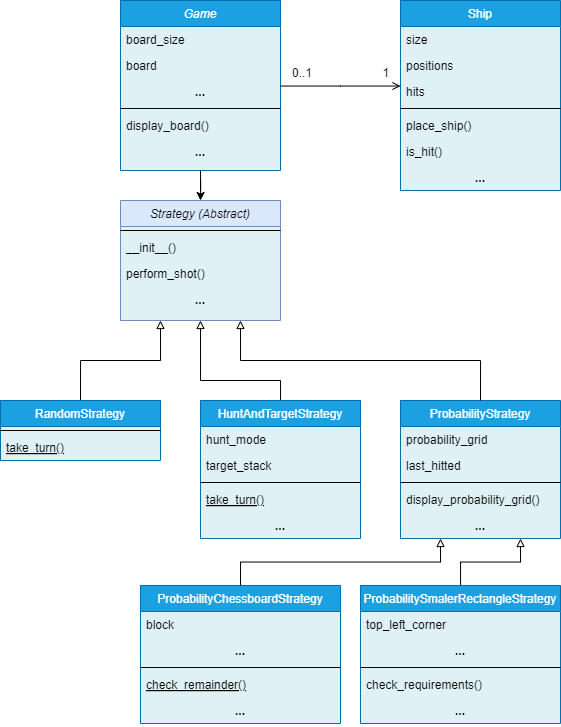
\includegraphics[width=0.8\textwidth]{diagram_klas_27_09.png} % wstaw swój plik
    \caption{Diagram klas projektu samodzielnie stworzony za pomocą narzędziea draw.io.} % podpis pod obrazkiem
    \label{fig:example} % etykieta do odniesienia w tekście
\end{figure}

Diagram klas ilustruje architekturę systemu gry strategicznej, w której klasa $Game$ pełni centralną rolę zarządcy całej rozgrywki. Każda instancja klasy $Game$ musi mieć przypisaną dokładnie jedną strategię, co jest realizowane za pomocą współpracy z klasą abstrakcyjną $Strategy$. Strategia jest kluczowym komponentem gry, ponieważ wpływa na logikę podejmowanych decyzji, takich jak wybór miejsca oddania strzału. Abstrakcyjna klasa $Strategy$ definiuje wspólne metody i właściwości dla wszystkich strategii, a konkretne implementacje strategii różnią się sposobem działania.
\newline
Klasa $Game$ posiada relację typu \textbf{jeden do wielu} z klasą $Ship$, co oznacza, że w ramach jednej gry może być przypisanych od jednego do wielu statków. Zgodnie z założeniami gry, do każdej instancji rozgrywki przypisanych jest dokładnie 5 statków, każdy o ściśle określonej wielkości.
\newline
Klasa $Strategy$ jest klasą abstrakcyjną, z której dziedziczą trzy różne strategie: $RandomStrategy$ (strategia losowa), $HuntAndTargetStrategy$ (strategia strzelania po trafieniu) oraz $ProbabilityStrategy$ (strategia probabilistyczna). Każda z tych strategii implementuje zgodnie z przedstawionymi wcześniejszym rozdziale różne podejścia do wyboru ruchu w grze.
\newline
Dodatkowo dwie podklasy $ProbabilityChessboardStrategy$ oraz 
\newline
$ProbabilitySmallerRectangleStrategy$ – dziedziczą bezpośrednio po klasie $ProbabilityStrategy$ i rozwijają jej zaawansowaną logikę opartą na różnych podejściach do obliczania prawdopodobieństwa. 
\newline
Taka struktura systemu zapewnia dużą elastyczność w definiowaniu różnych strategii rozgrywki oraz ułatwia rozszerzanie gry o potencjalnie nowe strategie w przyszłości.

\section{Słownik Danych}
Słownik danych określa zawartość klas w projekcie poprzez szczegółowy opis atrybutów oraz metod. Każda klasa jest opisana w kontekście jej roli w systemie, atrybuty definiują jej właściwości, natomiast metody przedstawiają operacje, które dana klasa może wykonywać. Słownik obejmuje klasy takie jak $Game$, $Ship$ oraz różne strategie, dostarczając informacji o ich funkcjach, dzięki temu możliwe jest pełne zrozumienie struktury oraz logiki implementacji systemu.
\subsection{Klasa Game}
\begin{table}[H]
\centering
\begin{tabularx}{\textwidth}{|p{6cm}|X|}
\hline
\textbf{Pojęcie i Typ} & \textbf{Zawartość} \\ \hline
\textbf{Klasa:} \texttt{Game} & Klasa reprezentująca rozgrywkę w grze statków. \\ \hline
\textbf{Atrybut:} \texttt{board\_size int} & Rozmiar planszy do gry (domyślnie 10). \\ \hline
\textbf{Atrybut:} \texttt{board list[list[str]]} & Dwuwymiarowa lista reprezentująca planszę gry (pola gry). \\ \hline
\textbf{Atrybut:} \texttt{ships list[Ship]} & Lista statków umieszczonych na planszy. \\ \hline
\textbf{Atrybut:} \texttt{shot\_count int} & Licznik oddanych strzałów. \\ \hline
\textbf{Atrybut:} \texttt{strategy Strategy} & Obiekt strategii używany do wykonywania ruchów w grze (domyślnie \texttt{RandomStrategy}). \\ \hline
\textbf{Atrybut:} \texttt{shots list[tuple[int, int]]} & Lista zawierająca wszystkie oddane strzały w formie krotek (wiersz, kolumna). \\ \hline
\textbf{Metoda:} \texttt{\_\_init\_\_(board\_size=10, strategy=None)} & Konstruktor inicjujący grę z domyślnym rozmiarem planszy i strategią. \\ \hline
\textbf{Metoda:} \texttt{display\_board(reveal=False)} & Wyświetla planszę, opcjonalnie pokazując ukryte statki. \\ \hline
\textbf{Metoda:} \texttt{add\_ship(size)} & Dodaje statek o określonym rozmiarze do planszy. \\ \hline
\textbf{Metoda:} \texttt{random\_position()} & Zwraca losową pozycję na planszy w formie krotki (wiersz, kolumna). \\ \hline
\textbf{Metoda:} \texttt{take\_shot(row, col)} & Wykonuje strzał w podanej pozycji; zwraca wynik strzału (trafienie, zatopienie). \\ \hline
\textbf{Metoda:} \texttt{is\_within\_bounds(row, col)} & Sprawdza, czy dana pozycja mieści się w granicach planszy. \\ \hline
\textbf{Metoda:} \texttt{is\_already\_shot(row, col)} & Sprawdza, czy w podanej pozycji już oddano strzał. \\ \hline
\textbf{Metoda:} \texttt{check\_hit(row, col)} & Sprawdza, czy strzał trafił w statek; zwraca wynik trafienia i zatopienia statku. \\ \hline
\textbf{Metoda:} \texttt{is\_game\_over()} & Sprawdza, czy wszystkie statki zostały zatopione (gra się skończyła). \\ \hline
\textbf{Metoda:} \texttt{start\_game(ship\_sizes)} & Rozpoczyna grę, dodając statki na planszę zgodnie z podanymi rozmiarami. \\ \hline
\end{tabularx}
\caption{Tabela przedstawiająca metody oraz atrybuty klasy Game.}
\end{table}

Klasa $Game$ jest centralnym elementem projektu, odpowiadającym za zarządzanie przebiegiem gry. Obsługuje planszę, rozmieszczanie statków, kontroluje liczbę oddanych strzałów oraz sprawdza, czy gra się zakończyła. Jest również odpoweidzialna za wybranie strategii.
\subsection{Klasa Ship}
\begin{table}[H]
\centering
\begin{tabularx}{\textwidth}{|p{6cm}|X|}
\hline
\textbf{Pojęcie i Typ} & \textbf{Zawartość} \\ \hline
\textbf{Klasa:} \texttt{Ship} & Klasa reprezentująca statek. \\ \hline
\textbf{Atrybut:} \texttt{size} & Rozmiar statku, czyli liczba pól, które zajmuje. \\ \hline
\textbf{Atrybut:} \texttt{positions} & Lista zawierająca współrzędne w postaci krotek (wiersz, kolumna) zajmowane przez statek na planszy. \\ \hline
\textbf{Atrybut:} \texttt{hits } & Liczba trafień, które statek otrzymał. \\ \hline
\textbf{Metoda:} \texttt{\_\_init\_\_(size)} & Konstruktor inicjujący statek z określonym rozmiarem. \\ \hline
\textbf{Metoda:} \texttt{place\_ship(board, start\_row, start\_col, direction) } & Umieszcza statek na planszy. \\ \hline
\textbf{Metoda:} \texttt{is\_hit(row, col)} & Sprawdza, czy statek został trafiony. \\ \hline
\textbf{Metoda:} \texttt{is\_sunk()} & Sprawdza, czy statek został zatopiony. \\ \hline
\textbf{Metoda:} \texttt{is\_damaged()} & Sprawdza, czy statek jest uszkodzony (trafiony, ale nie zatopiony). \\ \hline
\end{tabularx}
\caption{Tabela przedstawiająca klasę Ship z atrybutami oraz metodami.}
\end{table}



Klasa $Ship$ odpowiada za modelowanie statków w grze. Każdy statek ma określony rozmiar oraz pozycje na planszy, a także śledzi liczbę trafień. Metoda ${is\_hit(row, col)$ ma na celu sprawdzenie, czy statek znajdujący się na danym polu (określonym przez współrzędne row i col) został trafiony. Zwraca wartość logiczną: $True$, jeśli statek na tych współrzędnych został trafiony, lub $False$, jeśli nie. Dodatkowo, w przypadku trafienia, zwiększa licznik trafień(zostaje zwiększony atrubut $hits$ o jeden. Matomiast metody $is\_sunk$  porównuje liczbę trafień z rozmiarem statku. Jeśli liczba trafień jest równa rozmiarowi, zwraca True, co oznacza, że statek został zatopiony. W przeciwnym razie zwraca False. Ostatnia metoda $is\_damaged$ sprawdza czy statek został uszkodzony, czyli czy otrzymał przynajmniej jedno trafienie, ale nie został jeszcze zatopiony. Zwraca $True$, jeśli liczba trafień jest większa od zera, ale mniejsza niż rozmiar statku. W przeciwnym razie zwraca $False$.
\subsection{Klasa Strategy}
\begin{table}[H]
\centering
\begin{tabularx}{\textwidth}{|p{6cm}|X|}
\hline
\textbf{Pojęcie i Typ} & \textbf{Zawartość} \\ \hline
\textbf{Klasa:} \texttt{Strategy} & Abstrakcyjna klasa definiująca strategię gry. \\ \hline
\textbf{Atrybut:} \texttt{game} & Obiekt gry, do której odnosi się strategia. \\ \hline
\textbf{Metoda:} \texttt{\_\_init\_\_(game)} & Konstruktor inicjujący strategię z obiektem gry. \\ \hline
\textbf{Metoda:} \texttt{take\_turn()} & Abstrakcyjna metoda do realizacji tury (musi zostać zaimplementowana w klasach pochodnych). \\ \hline
\textbf{Metoda:} \texttt{select\_random\_shot()} & Wybiera losowy strzał na planszy, upewniając się, że nie był jeszcze wykonany. \\ \hline
\textbf{Metoda:} \texttt{add\_adjacent\_targets(row, col)} & Dodaje sąsiednie pola jako potencjalne cele do ataku. \\ \hline
\textbf{Metoda:} \texttt{perform\_shot(row, col)} & Wykonuje strzał w podanych współrzędnych i aktualizuje stan gry. \\ \hline
\end{tabularx}
\caption{Tabela przedstawiająca metody oraz atrybuty klasy Strategy.}
\end{table}

Klasa $Strategy$ będąca abstrakcyjną bazą dla wszystkich strategii gry, definiuje wspólne atrybuty oraz metody pomocnicze, takie jak wybór losowego strzału czy dodawanie sąsiednich celów. Metoda $take\_turn()$ pozostaje abstrakcyjna i musi być implementowana przez konkretne strategie.

Poniżej zostaną przedstawione tabele róźnych strategii, które zostały wykorzystane w przedstawionej analizie. Dokładny opis strategii oraz zasady na jakich one działają zostaną opisane w następnym rozdziale.
\subsection{Klasa RandomStrategy}
\begin{table}[H]
\centering
\begin{tabularx}{\textwidth}{|p{6cm}|X|}
\hline
\textbf{Pojęcie i Typ} & \textbf{Zawartość} \\ \hline
\textbf{Klasa:} \texttt{RandomStrategy} & Klasa reprezentująca strategię losowych strzałów. \\ \hline
\textbf{Metoda:} \texttt{take\_turn()} & Wybiera losowy strzał i aktualziuje planszę. \\ \hline
\end{tabularx}
\caption{Tabela przedstawiająca klasę RandomStrategy z metodami.}
\end{table}


Strategia $RandomStrategy$ implementuje metodę $take turn$, wykonując losowy strzał na planszy. Jest to najprostsza strategia, w której każda tura opiera się na losowym wyborze pozycji.
\subsection{Klasa HuntAndTargetStrategy}
Strategia $HuntAndTargetStrategy$ jest rozszerzeniem strategii losowej, która wprowadza dwa tryby działania:

Tryb polowania (hunt mode) – strzelanie w losowe miejsca, dopóki nie zostanie trafiony statek.
Tryb celu (target mode) – po trafieniu statku, dodawane są do listy sąsiednie pola, które stają się potencjalnymi celami kolejnych strzałów.
\subsection{Klasa ProbabilityStrategy}
\begin{table}[H]
\centering
\begin{tabularx}{\textwidth}{|p{6cm}|X|}
\hline
\textbf{Pojęcie i Typ} & \textbf{Zawartość} \\ \hline
\textbf{Klasa:} \texttt{ProbabilityStrategy} & Klasa implementująca strategię opartą na prawdopodobieństwie w grze. \\ \hline
\textbf{Atrybut:} \texttt{probability\_grid} & Dwuwymiarowa lista przechowująca prawdopodobieństwo, że statek znajduje się w danej komórce planszy. \\ \hline
\textbf{Atrybut:} \texttt{last\_hitted} & Lista przechowująca ostatnie trafione pola. \\ \hline
\textbf{Metoda:} \texttt{\_\_init\_\_(game)} & Konstruktor inicjujący strategię, tworzy macierz oceny strzału oraz listę ostatnich trafień. \\ \hline
\textbf{Metoda:} \texttt{display\_probability\_grid()} & Wyświetla macierz oceny strzału w konsoli. \\ \hline
\textbf{Metoda:} \texttt{update\_probability\_grid()} & Aktualizuje macierz oceny strzału na podstawie aktualnego stanu gry. \\ \hline
\textbf{Metoda:} \texttt{update\_probability\_grid\_not \_hitted\_ship()} & Aktualizuje macierz oceny strzału, gdy nie trafiono w żaden statek. \\ \hline
\textbf{Metoda:} \texttt{update\_probability\_grid \_hitted\_ship()} & Aktualizuje macierz oceny strzału w przypadku trafienia w statek. \\ \hline
\textbf{Metoda:} \texttt{probability\_shot()} & Wybiera komórkę o najwyższym prawdopodobieństwie i wykonuje strzał. \\ \hline
\textbf{Metoda:} \texttt{take\_turn()} & Aktualizuje macierz oceny strzału, wyświetla ją i wykonuje strzał. \\ \hline
\end{tabularx}
\caption{Tabela przedstawiająca klasę ProbabilityStrategy z atrybutami oraz metodami.}
\end{table}

Strategia $ProbabilityStrategy$ wykorzystuje tablicę prawdopodobieństw do szacowania najbardziej prawdopodobnych miejsc występowania statków, uwzględniając ich rozmiary i możliwe rozmieszczenie na planszy. Metody ${update\_probability\_grid()}$ \newline ${update\_probability\_grid\_not\_hitted\_ship() }$ oraz $ update\_probability\_grid\_hitted\_ship() $ odpowiadają za analizę i aktualizację macierzy oceny strzału w oparciu o to, czy statki zostały trafione czy nie. Dzięki tym metodom strategia jest w stanie dynamicznie reagować na wyniki strzałów i zmieniać swoje podejście do ataku.
\subsection{Klasa ProbabilityChessboardStrategy}
\begin{table}[H]
\centering
\begin{tabularx}{\textwidth}{|p{6cm}|X|}
\hline
\textbf{Pojęcie i Typ} & \textbf{Zawartość} \\ \hline
\textbf{Klasa:} \texttt{ProbabilityChessboard Strategy} & Klasa implementująca ulepszoną strategię opartą na prawdopodobieństwie oraz zasadach szachownicy w grze. \\ \hline
\textbf{Atrybut:} \texttt{block} & Parametr określający, w którym momencie zastosować strategię szachownicy. \\ \hline
\textbf{Atrybut:} \texttt{divisor} & Wartość używana do obliczeń reszty dla strategii szachownicy. \\ \hline
\textbf{Atrybut:} \texttt{remainder} & Oczekiwana reszta z operacji dzielenia, stosowana w strategii. \\ \hline
\textbf{Metoda:} \texttt{\_\_init\_\_(game, divisor, remainder, block)} & Konstruktor inicjujący strategię, ustawia wartości dla dzielnika, reszty oraz bloku. \\ \hline
\textbf{Metoda:} \texttt{check\_remainder(divisor, remainder, num1, num2)} & Sprawdza, czy suma dwóch liczb daje oczekiwaną resztę przy dzieleniu przez dzielnik. \\ \hline
\textbf{Metoda:} \texttt{update\_probability\_grid\_not \_hitted\_ship()} & Aktualizuje macierz oceny strzału, stosując strategię szachownicy, jeżeli liczba strzałów jest mniejsza niż wartość bloku; w przeciwnym razie stosuje normalną strategię. \\ \hline
\end{tabularx}
\caption{Tabela przedstawiająca klasę $ProbabilityChessboardStrategy$ z atrybutami oraz metodami.}
\end{table}
Klasa $ProbabilityChessboardStrategy$ rozszerza klasę $ProbabilityStrategy$ i implementuje zaawansowaną strategię opartą na prawdopodobieństwie, łącząc ją z zasadami szachownicy. Głównym celem tej klasy jest optymalizacja wyboru pól w pierwszych strzałach.Atrybuty $block$, $divisor$ i $remainder$ są kluczowe dla działania strategii szachownicy. Atrybut $block$ definiuje próg, po przekroczeniu którego strategia przestaje stosować zasady szachownicy. Atrybuty $divisor$ i $remainder$ są wykorzystywane do obliczeń, które decydują o tym, które pola mają być preferowane w pierwszej kolejności.
\subsection{Klasa ProbabilitySmallerRectangleStrategy}
\begin{table}[H]
\centering
\begin{tabularx}{\textwidth}{|p{6cm}|X|}
\hline
\textbf{Pojęcie i Typ} & \textbf{Zawartość} \\ \hline
\textbf{Klasa:} \texttt{ProbabilitySmallerRectangle Strategy} & Klasa implementująca ulepszoną strategię opartą na prawdopodobieństwie, koncentrującą się na mniejszych obszarach planszy. \\ \hline
\textbf{Atrybut:} \texttt{block} & Parametr określający, w którym momencie zastosować normalną strategię, gdy liczba strzałów osiągnie wartość bloku. \\ \hline
\textbf{Atrybut:} \texttt{top\_left\_corner} & Współrzędne lewego górnego rogu mniejszego kwadratu, w którym strategia będzie koncentrować swoje strzały. \\ \hline
\textbf{Atrybut:} \texttt{lower\_right\_corner} & Współrzędne prawego dolnego rogu mniejszego kwadratu, w którym strategia będzie koncentrować swoje strzały. \\ \hline
\textbf{Metoda:} \texttt{\_\_init\_\_(game, top\_left\_corner, lower\_right\_corner, block)} & Konstruktor inicjujący strategię, ustawiający wartości dla bloku oraz współrzędnych rogów. \\ \hline
\textbf{Metoda:} \texttt{check\_requirements( top\_left\_corner, lower\_right\_corner, position)} & Sprawdza, czy dana pozycja znajduje się wewnątrz określonego mniejszego kwadratu. \\ \hline
\textbf{Metoda:} \texttt{update\_probability\_grid\_not \_hitted\_ship()} & Aktualizuje macierz oceny strzału, stosując strategię mniejszego kwadratu, jeśli liczba strzałów jest mniejsza niż wartość bloku; w przeciwnym razie wywołuje normalną strategię. \\ \hline
\end{tabularx}
\caption{Tabela przedstawiająca klasę $ProbabilitySmallerRectangleStrategy$ z atrybutami oraz metodami.}
\end{table}
Klasa $ProbabilitySmallerRectangleStrategy$ analogicznie jak wcześniejsza klasa rozszerza klasę $ProbabilityStrategy$ i wprowadza zaawansowaną strategię opartą na prawdopodobieństwie, skupiając się na konkretnych, mniejszych obszarach planszy w celu optymalizacji strzałów. Strategia ta ma na celu zwiększenie efektywności ataków na wyznaczonym prostokątnym obszarze.
\chapter{Złożoność algorytmów}
W tym rozdziale zostanie przedstawione, jak obliczyć złożoność obliczeniową przy inicjalizacji gry ze statkami o długościach [2, 3, 3, 4, 5] oraz wybraniu ustalonej strategii opisanej we wcześniejszych rozdziałach. Każda gra, niezależnie od wyboru strategii, musi wygenerować planszę oraz dodać statki przy użyciu metody \texttt{add\_ship()}. Niech $n$ będzie długością planszy. Wtedy przy inicjalizacji planszy (macierz $n \times n$) mamy złożoność obliczeniową:

$$
O(n^2).
$$

Dodanie pięciu statków o długościach [2, 3, 3, 4, 5] przy użyciu metody \texttt{add\_ship()} można oszacować jako:

$$
O(\text{liczba statków} \cdot n^2) = O(5 \cdot n^2),
$$

co po pominięciu stałej daje złożoność rzędu:

$$
O(n^2).
$$

Złożoność obliczeniowa przed wykonaniem pierwszego ruchu w najgorszym przypadku wynosi:

$$
O(n^4).
$$

W kolejnych rozdziałach zostanie przedstawione obliczenie złożoności poszczególnych strategii dla jednego ruchu.
\section{Złożoność dla strategii losowej}
Algorytm zawarty w klasie $RandomStrategy$ opiera się na losowym wyborze współrzędnych strzału. Funkcja $select\_random\_shot()$ losowo wybiera współrzędne $(row, col)$ na planszy o wymiarach $n \times n$, aż znajdzie pozycję, która nie została jeszcze wybrana (czyli nie występuje w atrybucie $shots$ dla Klasy $Game$. W najgorszym przypadku, gdy pozostało jedno wolne pole, funkcja może iterować aż $O(n^2)$ razy, aby znaleźć wolne miejsce.

Zatem złożoność wyboru strzału w najgorszym scenariuszu wynosi:
$$
O(n^2).
$$

Zakładając, że gra trwa maksymalnie $O(n^2)$ tur (tyle jest możliwych strzałów na planszy o wymiarach $n \times n$), łączna złożoność algorytmu dla całej gry wynosi:
$$
O(n^2) \times O(n^2) = O(n^4).
$$
\section{Złożoność dla strategii "strzelania po trafieniu"}
\section{Złożoność strategii probabilistycznych}
Algorytm składa się z dwóch kluczowych kroków: aktualizacji macierzy prawdopodobieństw oceny strzału oraz wykonania strzału opartego na tej macierzy. Proces aktualizacji macierzy prawdopodobieństw może przebiegać w dwóch scenariuszach:

\begin{itemize}
  \item Dla nieuszkodzonych statków funkcja iteruje przez wszystkie możliwe pozycje na planszy, sprawdzając, gdzie można potencjalnie umieścić statki. Dla każdego statku iteracja odbywa się po planszy o wymiarach $n \times n$, co oznacza, że dla pojedynczego statku złożoność wynosi $O(n^2)$. Jeśli mamy $k$ statków, złożoność można oszacować jako:
  $$
  O(k \cdot n^2).
  $$
  W przypadku typowej gry, w której liczba statków jest stała (na przykład 5 statków), złożoność upraszcza się do:
  $$
  O(5 \cdot n^2) = O(n^2).
  $$

  \item W przypadku uszkodzenia, ale niezatopienia statku algorytm koncentruje się na sąsiadujących polach, aby zlokalizować pozostałe części uszkodzonego statku. W najgorszym scenariuszu, gdy algorytm musi przeanalizować większy obszar planszy, złożoność pozostaje taka sama jak w przypadku braku trafionych statków, czyli:
  $$
  O(k \cdot n^2) = O(n^2).
  $$ 
\end{itemize}

Niezależnie od tego, czy któryś ze statków został trafiony, czy nie, aktualizacja macierzy prawdopodobieństw ma złożoność rzędu $O(n^2)$.

Następnym krokiem algorytmu jest wykonanie strzału, który opiera się na zaktualizowanej macierzy prawdopodobieństw. Funkcja \texttt{probability\_shot()} iteruje po całej macierzy, aby znaleźć komórkę z najwyższym prawdopodobieństwem trafienia, co ma złożoność:
$$
O(n^2).
$$

Zatem łączna złożoność dla pojedynczego ruchu, obejmująca zarówno aktualizację macierzy, jak i wykonanie strzału, wynosi:
$$
O(n^2) + O(n^2) = O(n^2).
$$
Jeśli jednak rozpatrujemy pełną grę, w której funkcje te są wywoływane wielokrotnie (w każdej turze), złożoność algorytmu rośnie. Zakładając, że gra może trwać około $O(n^2)$ tur, łączna złożoność dla całej gry wynosi:
$$
O(n^2) \times O(n^2) = O(n^4).
$$

Dla strategii dziedziczących po $ProbabilityStrategy$, takich jak \newline $ProbabilityChessboardStrategy$ oraz $ProbabilitySmallerRectangleStrategy$, złożoność metody $update\_probability\_grid\_not\_hitted\_ship()$ różni się nieco od podstawowej wersji algorytmu. W tych strategiach wprowadzono dodatkowe kryteria filtrowania pól planszy, jak na przykład sprawdzanie reszty z dzielenia sumy indeksów wierszy i kolumn bądź ograniczenie obszaru przeszukiwania do mniejszego prostokąta. 

Proces przeglądania wszystkich niezatopionych statków, zarówno w pionie, jak i poziomie, zachowuje złożoność rzędu:
$$
O(k \cdot n^2) = O(n^2).
$$
Dodatkowe operacje filtrowania są wykonywane na poszczególnych polach i mają złożoność rzędu:
$$
O(1).
$$
Dlatego ogólna złożoność dla tych strategii nie różni się znacząco od bazowej strategii \newline $ProbabilityStrategy$ i wynosi $O(n^2)$ na turę, natomaist w kontekście całej rozgrywki wynosi $O(n^4)$.
\chapter{Testy}

\section{Analiza statystyczna dla strategii losowej}
\section{Analiza statystyczna dla strategii "strzelania po trafieniu"}
\section{Analiza statystyczna dla strategii probabilistycznej}
\section{Analiza statystyczna dla strategii probabilistycznej z użyciem szachownicy}
\section{Analiza statystyczna dla strategii probabilistycznej ograniczenego obszaru}
\section{Porówananie pierwszych trzech strategii}
\section{Porówananie strategii probabilistycznych: klasycznej z szachownicą}
\section{Porówananie strategii probabilistycznych: klasycznej z ograniczonym obszarem}
\chapter{Wnioski}
\begin{thebibliography}{9}
  \addcontentsline{toc}{chapter}{Bibliografia}
  \bibitem{Statystyka_1} 
  Koronacki, Jacek, Mielniczuk, Jan. 
  \textit{Statystyka dla studentów kierunków technicznych i przyrodniczych}. 
  Warszawa: Wydawnictwo Naukowo-Techniczne, 2001.
  \bibitem{Statystyka_2} 
  Jakubowski, Jacek, Sztencel, Rafał. 
  \textit{Wstęp do teorii prawdopodobieństwa.}. 
  Warszawa: Wydawnictwo Script, 2001.
  \bibitem{yt_1} 
  @digitalgenius111. 
  \textit{How to 'always' win at Battleship?}. 
  [Online]. Available: https://www.youtube.com/watch?v=8FctDuTfcO8. 
  [Dostęp: 28.09.2024].
  
  \end{thebibliography}
  
\end{document}
